\documentclass[a4paper,12pt,fleqn]{article}%fleqn pour aligner les equations à gauche
\usepackage{/home/rweye/Documents/Overleaf/Styles/Cours}

\title{\vspace{-1cm}\large 
	\begin{tabular}{|>{\centering}m{5cm}|>{\centering}m{8cm}|>{\centering\arraybackslash}m{4cm}|}
		\hline
		Activité 1 & \textbf{\textsc{La Terre, seule planète habitable ?}} &  Chapitre 5 \\
		\hline
\end{tabular}
\vspace{-5em}}
\date{}

\begin{document}
\maketitle
\noindent Les deux tiers de la Terre sont couverts par des mers et des océans. L'eau liquide, qui constitue environ \SI{70}{\percent} des êtres vivants, set la source de la vie que nous connaissons. Pourtant occupons-nous la seule planète habitée ?

\begin{figure}[h!]
\caption{\textbf{L'eau liquide, condition fondamentale pour le développement de la vie}}
\begin{multicols}{2}
Des études expérimentales ont permis de déterminer l'état de l'eau pour toutes les conditions de pressions et températures possibles : c'est le diagramme de phase (attention, dans le graphique ci-dessous, l'échelle des donnée est logarithmique).\\

\begin{minipage}{.5\textwidth}
\begin{center}
	\textbf{Diagramme de phase de l'eau}
	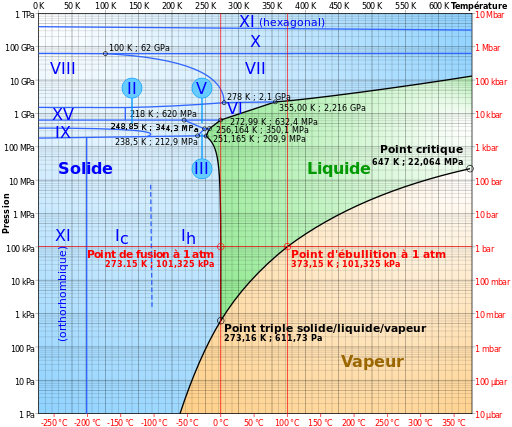
\includegraphics[width=\linewidth]{Ressources/1ES_C5_Act1_Fig2.png}
\end{center}
\end{minipage}

\begin{minipage}{\linewidth}
\begin{center}
	\textbf{Conditions de surface de la Terre, la Lune et Mars}
	\begin{tabular}{|>{\centering}m{.25\linewidth}|>{\centering}m{.2\linewidth}|>{\centering}m{.2\linewidth}|>{\centering\arraybackslash}m{.2\linewidth}|}
	\hline
	\textbf{Astre} 	& \textbf{Terre} & \textbf{Lune} & \textbf{Mars}\\
	\hline \textbf{Température} & \num{-90} à \SI{+60}{\celsius} &\num{-247} à \SI{+120}{\celsius} & \num{-143} à \SI{+20}{\celsius}\\
	\hline \textbf{Pression atmosphérique} & \SI{1E5}{Pa} Eau : non &\SI{3E-10}{Pa} Eau : non & \SI{600}{Pa} Eau : oui\\
	\hline 
	\end{tabular}
\end{center}
\end{minipage}

\vspace{1em}
\begin{minipage}{\linewidth}
\textbf{Région de Reull Vallis sur la planète Mars}\\
La sonde Raven a montré que le vent solaire a emporté une grande partie de l'atmosphère martienne.
\begin{center}
	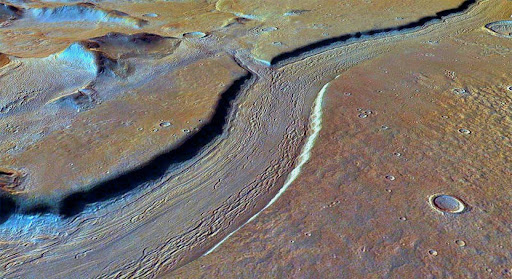
\includegraphics[width=.8\linewidth]{Ressources/1ES_C5_Act1_Fig3.jpg}
\end{center}
\end{minipage}
\end{multicols}
\end{figure}

\begin{figure}[h!]
\begin{multicols}{2}
\caption{\textbf{Zone d'habitabilité et vie extraterrestre}}
Les pressions et températures des exoplanètes sont aujourd'hui  inaccessibles. La température est estimée en fonction de la puissance de l'étoile (corrélée à sa masse) et de la distance à l'étoile. Une gravité suffisante est nécessaire pour avoir une atmosphère et donc un éventuel effet de serre. On définit une \textit{zone habitable}, comme la région autour d'une étoile où l'eau éventuelle peut être liquide.
\begin{center}
	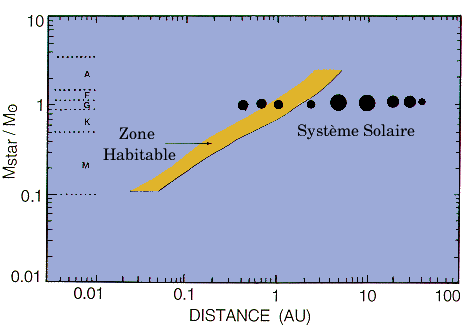
\includegraphics[width=\linewidth]{Ressources/1ES_C5_Act1_Fig1.png}
\end{center}
\columnbreak
\caption{\textbf{Des exoplanètes habitées ?}}
Des milliers d'exoplanètes ont été recensées depuis 1995. Leurs caractéristiques sont étudiées grâce à des télescopes puissants permettant d'analyser les espèces chimiques en fonction de spectrogrammes.\\
K2-18b possède les signatures spectrales de \ce{H2O}, \ce{CO2}, \ce{CH4} et \ce{DMS} (diméthylesulfide), une molécule produite par le phytoplancton sur Terre.
\begin{center}
	\begin{tabular}{|>{\centering}m{.25\linewidth}|>{\centering}m{.1\linewidth}|>{\centering}m{.15\linewidth}|>{\centering}m{.15\linewidth}|>{\centering\arraybackslash}m{.15\linewidth}|}
	\hline
	\textbf{Astre étudié}&\textbf{Terre} & \textbf{K2-18b}& \textbf{Kepler 22b}& \textbf{TOI-1489 b}\\
	\hline
	\textbf{Nom de l'étoile} & Soleil & K2-1 & Kepler & Gliese 892\\
	\hline \small $\dfrac{M_{etoile}}{M_{Soleil}}$ & 1 & 0,4 & 0,97 & 0,8\\
	\hline
	\textbf{Distance à l'étoile} & \SI{1}{U.A.} & \SI{0,14}{U.A.} & \SI{0,85}{U.A.} & \SI{0,04}{U.A.}\\
	\hline
	\textbf{Signature spectrale de l'eau} & oui & oui & ? & ?\\
	\hline 
	\textbf{Atmosphère} & oui & oui & oui & inconnue\\
	\hline
	\textbf{Température moyenne} & \num{-90} à \SI{+60}{\celsius} & \num{-23} à \SI{+27}{\celsius} &  \SI{21}{\celsius} $\pm$ \SI{55}{\celsius} & \SI{-104}{\celsius}\\
	\hline
	\end{tabular}
\end{center}
\end{multicols}
\end{figure}

\begin{enumerate}
	\item Placer la Terre, Mars et la Lune sur diagramme de phase. Conclure sur la présence d'eau liquide.
	\item Proposer une hypothèse à l'observation de vallées creusées par l'eau sur Mars.
	\item Lister les critères à prendre en compte pour estimer le caractère habitable d'une planète.
	\item Identifier la ou les exoplanètes susceptibles d'être habitables. Argumenter.
\end{enumerate}

\end{document}